\documentclass[]{ctexbook}
\usepackage{lmodern}
\usepackage{amssymb,amsmath}
\usepackage{ifxetex,ifluatex}
\usepackage{fixltx2e} % provides \textsubscript
\ifnum 0\ifxetex 1\fi\ifluatex 1\fi=0 % if pdftex
  \usepackage[T1]{fontenc}
  \usepackage[utf8]{inputenc}
\else % if luatex or xelatex
  \ifxetex
    \usepackage{xltxtra,xunicode}
  \else
    \usepackage{fontspec}
  \fi
  \defaultfontfeatures{Ligatures=TeX,Scale=MatchLowercase}
\fi
% use upquote if available, for straight quotes in verbatim environments
\IfFileExists{upquote.sty}{\usepackage{upquote}}{}
% use microtype if available
\IfFileExists{microtype.sty}{%
\usepackage{microtype}
\UseMicrotypeSet[protrusion]{basicmath} % disable protrusion for tt fonts
}{}
\usepackage[b5paper,tmargin=2.5cm,bmargin=2.5cm,lmargin=3.5cm,rmargin=2.5cm]{geometry}
\usepackage[unicode=true]{hyperref}
\PassOptionsToPackage{usenames,dvipsnames}{color} % color is loaded by hyperref
\hypersetup{
            pdftitle={Overleaf功能介绍},
            pdfauthor={wang},
            colorlinks=true,
            linkcolor=Maroon,
            citecolor=Blue,
            urlcolor=Blue,
            breaklinks=true}
\urlstyle{same}  % don't use monospace font for urls
\usepackage{natbib}
\bibliographystyle{apalike}
\usepackage{color}
\usepackage{fancyvrb}
\newcommand{\VerbBar}{|}
\newcommand{\VERB}{\Verb[commandchars=\\\{\}]}
\DefineVerbatimEnvironment{Highlighting}{Verbatim}{commandchars=\\\{\}}
% Add ',fontsize=\small' for more characters per line
\usepackage{framed}
\definecolor{shadecolor}{RGB}{248,248,248}
\newenvironment{Shaded}{\begin{snugshade}}{\end{snugshade}}
\newcommand{\AlertTok}[1]{\textcolor[rgb]{0.94,0.16,0.16}{#1}}
\newcommand{\AnnotationTok}[1]{\textcolor[rgb]{0.56,0.35,0.01}{\textbf{\textit{#1}}}}
\newcommand{\AttributeTok}[1]{\textcolor[rgb]{0.77,0.63,0.00}{#1}}
\newcommand{\BaseNTok}[1]{\textcolor[rgb]{0.00,0.00,0.81}{#1}}
\newcommand{\BuiltInTok}[1]{#1}
\newcommand{\CharTok}[1]{\textcolor[rgb]{0.31,0.60,0.02}{#1}}
\newcommand{\CommentTok}[1]{\textcolor[rgb]{0.56,0.35,0.01}{\textit{#1}}}
\newcommand{\CommentVarTok}[1]{\textcolor[rgb]{0.56,0.35,0.01}{\textbf{\textit{#1}}}}
\newcommand{\ConstantTok}[1]{\textcolor[rgb]{0.00,0.00,0.00}{#1}}
\newcommand{\ControlFlowTok}[1]{\textcolor[rgb]{0.13,0.29,0.53}{\textbf{#1}}}
\newcommand{\DataTypeTok}[1]{\textcolor[rgb]{0.13,0.29,0.53}{#1}}
\newcommand{\DecValTok}[1]{\textcolor[rgb]{0.00,0.00,0.81}{#1}}
\newcommand{\DocumentationTok}[1]{\textcolor[rgb]{0.56,0.35,0.01}{\textbf{\textit{#1}}}}
\newcommand{\ErrorTok}[1]{\textcolor[rgb]{0.64,0.00,0.00}{\textbf{#1}}}
\newcommand{\ExtensionTok}[1]{#1}
\newcommand{\FloatTok}[1]{\textcolor[rgb]{0.00,0.00,0.81}{#1}}
\newcommand{\FunctionTok}[1]{\textcolor[rgb]{0.00,0.00,0.00}{#1}}
\newcommand{\ImportTok}[1]{#1}
\newcommand{\InformationTok}[1]{\textcolor[rgb]{0.56,0.35,0.01}{\textbf{\textit{#1}}}}
\newcommand{\KeywordTok}[1]{\textcolor[rgb]{0.13,0.29,0.53}{\textbf{#1}}}
\newcommand{\NormalTok}[1]{#1}
\newcommand{\OperatorTok}[1]{\textcolor[rgb]{0.81,0.36,0.00}{\textbf{#1}}}
\newcommand{\OtherTok}[1]{\textcolor[rgb]{0.56,0.35,0.01}{#1}}
\newcommand{\PreprocessorTok}[1]{\textcolor[rgb]{0.56,0.35,0.01}{\textit{#1}}}
\newcommand{\RegionMarkerTok}[1]{#1}
\newcommand{\SpecialCharTok}[1]{\textcolor[rgb]{0.00,0.00,0.00}{#1}}
\newcommand{\SpecialStringTok}[1]{\textcolor[rgb]{0.31,0.60,0.02}{#1}}
\newcommand{\StringTok}[1]{\textcolor[rgb]{0.31,0.60,0.02}{#1}}
\newcommand{\VariableTok}[1]{\textcolor[rgb]{0.00,0.00,0.00}{#1}}
\newcommand{\VerbatimStringTok}[1]{\textcolor[rgb]{0.31,0.60,0.02}{#1}}
\newcommand{\WarningTok}[1]{\textcolor[rgb]{0.56,0.35,0.01}{\textbf{\textit{#1}}}}
\usepackage{longtable,booktabs}
% Fix footnotes in tables (requires footnote package)
\IfFileExists{footnote.sty}{\usepackage{footnote}\makesavenoteenv{long table}}{}
\IfFileExists{parskip.sty}{%
\usepackage{parskip}
}{% else
\setlength{\parindent}{0pt}
\setlength{\parskip}{6pt plus 2pt minus 1pt}
}
\setlength{\emergencystretch}{3em}  % prevent overfull lines
\providecommand{\tightlist}{%
  \setlength{\itemsep}{0pt}\setlength{\parskip}{0pt}}
\setcounter{secnumdepth}{5}
% Redefines (sub)paragraphs to behave more like sections
\ifx\paragraph\undefined\else
\let\oldparagraph\paragraph
\renewcommand{\paragraph}[1]{\oldparagraph{#1}\mbox{}}
\fi
\ifx\subparagraph\undefined\else
\let\oldsubparagraph\subparagraph
\renewcommand{\subparagraph}[1]{\oldsubparagraph{#1}\mbox{}}
\fi

% set default figure placement to htbp
\makeatletter
\def\fps@figure{htbp}
\makeatother

\usepackage{booktabs}
\usepackage{longtable}

\usepackage{framed,color}
\definecolor{shadecolor}{RGB}{248,248,248}

\renewcommand{\textfraction}{0.05}
\renewcommand{\topfraction}{0.8}
\renewcommand{\bottomfraction}{0.8}
\renewcommand{\floatpagefraction}{0.75}

\let\oldhref\href
\renewcommand{\href}[2]{#2\footnote{\url{#1}}}

\makeatletter
\newenvironment{kframe}{%
\medskip{}
\setlength{\fboxsep}{.8em}
 \def\at@end@of@kframe{}%
 \ifinner\ifhmode%
  \def\at@end@of@kframe{\end{minipage}}%
  \begin{minipage}{\columnwidth}%
 \fi\fi%
 \def\FrameCommand##1{\hskip\@totalleftmargin \hskip-\fboxsep
 \colorbox{shadecolor}{##1}\hskip-\fboxsep
     % There is no \\@totalrightmargin, so:
     \hskip-\linewidth \hskip-\@totalleftmargin \hskip\columnwidth}%
 \MakeFramed {\advance\hsize-\width
   \@totalleftmargin\z@ \linewidth\hsize
   \@setminipage}}%
 {\par\unskip\endMakeFramed%
 \at@end@of@kframe}
\makeatother

\makeatletter
\@ifundefined{Shaded}{
}{\renewenvironment{Shaded}{\begin{kframe}}{\end{kframe}}}
\@ifpackageloaded{fancyvrb}{%
  % https://github.com/CTeX-org/ctex-kit/issues/331
  \RecustomVerbatimEnvironment{Highlighting}{Verbatim}{commandchars=\\\{\},formatcom=\xeCJKVerbAddon}%
}{}
\makeatother

\usepackage{makeidx}
\makeindex

\urlstyle{tt}

\usepackage{amsthm}
\makeatletter
\def\thm@space@setup{%
  \thm@preskip=8pt plus 2pt minus 4pt
  \thm@postskip=\thm@preskip
}
\makeatother

\frontmatter

\title{Overleaf功能介绍}
\author{wang}
\date{2019-05-31}

\let\BeginKnitrBlock\begin \let\EndKnitrBlock\end
\begin{document}
\maketitle


\thispagestyle{empty}

\begin{center}
献给……

呃,爱谁谁吧
\end{center}

\setlength{\abovedisplayskip}{-5pt}
\setlength{\abovedisplayshortskip}{-5pt}

{
\setcounter{tocdepth}{2}
\tableofcontents
}
\listoftables
\listoffigures
\hypertarget{section}{%
\chapter*{前言}\label{section}}


Overleaf是什么

\url{https://www.overleaf.com/}

简单讲,Overleaf是一个在线的LaTeX环境.
不需要在自己电脑上安装,通过网页访问即可编写LaTeX.

如果还不了解LaTeX,可以先阅读下面的链接:

LaTeX的介绍:
\url{https://liam.page/2014/09/08/latex-introduction/}

当然,Overleaf提供的服务远不止此.

借助Overleaf,可以实现多人合作编辑,无缝同步进度,追踪文件修改历史.

你好,世界。我写了一本书。这本书是这样的,第 \ref{intro} 章介绍了啥啥,第 \ref{wind} 章说了啥啥,然后是啥啥\ldots{}\ldots{}

我用了两个 R 包编译这本书,分别是 \textbf{knitr}\index{knitr} \citep{xie2015} 和 \textbf{bookdown}\index{bookdown} \citep{R-bookdown}。以下是我的 R 进程信息:

\begin{Shaded}
\begin{Highlighting}[]
\KeywordTok{sessionInfo}\NormalTok{()}
\end{Highlighting}
\end{Shaded}

\begin{verbatim}
## R version 3.6.0 (2019-04-26)
## Platform: x86_64-apple-darwin15.6.0 (64-bit)
## Running under: macOS Mojave 10.14.4
## 
## Matrix products: default
## BLAS:   /Library/Frameworks/R.framework/Versions/3.6/Resources/lib/libRblas.0.dylib
## LAPACK: /Library/Frameworks/R.framework/Versions/3.6/Resources/lib/libRlapack.dylib
## 
## locale:
## [1] en_US.UTF-8/en_US.UTF-8/en_US.UTF-8/C/en_US.UTF-8/en_US.UTF-8
## 
## attached base packages:
## [1] stats     graphics  grDevices utils     datasets 
## [6] methods   base     
## 
## loaded via a namespace (and not attached):
##  [1] compiler_3.6.0  magrittr_1.5    bookdown_0.11  
##  [4] tools_3.6.0     htmltools_0.3.6 rstudioapi_0.10
##  [7] yaml_2.2.0      Rcpp_1.0.1      stringi_1.4.3  
## [10] rmarkdown_1.13  highr_0.8       knitr_1.23     
## [13] stringr_1.4.0   xfun_0.7        digest_0.6.18  
## [16] xtable_1.8-4    evaluate_0.14
\end{verbatim}

\hypertarget{section-1}{%
\section*{致谢}\label{section-1}}


非常感谢谁谁以及谁谁对我的帮助。艾玛,要不是他们神一样的队友,我两年前就写完这本书了。

\BeginKnitrBlock{flushright}
张三\\
于 A 村某角落
\EndKnitrBlock{flushright}

\hypertarget{author}{%
\chapter*{作者简介}\label{author}}


上不了厅堂,下得了厨房。敲得了代码,逮得住蟑螂。

\mainmatter

\hypertarget{intro}{%
\chapter{Overleaf写作流程}\label{intro}}

\hypertarget{section-2}{%
\section{创建项目}\label{section-2}}

空白文档
GitHub
\ldots{}

\hypertarget{section-3}{%
\section{个人写作}\label{section-3}}

\hypertarget{section-4}{%
\section{邀请合作者}\label{section-4}}

\hypertarget{section-5}{%
\section{论文投递}\label{section-5}}

现在我们可以试试 \textbf{bookdown} 的一些初级功能了,例如图表。图 \ref{fig:hello} 是一幅无趣的散点图,表 \ref{tab:iris} 是一份枯燥的数据。

\begin{Shaded}
\begin{Highlighting}[]
\KeywordTok{par}\NormalTok{(}\DataTypeTok{mar =} \KeywordTok{c}\NormalTok{(}\DecValTok{4}\NormalTok{, }\DecValTok{4}\NormalTok{, }\DecValTok{1}\NormalTok{, }\FloatTok{.1}\NormalTok{))}
\KeywordTok{plot}\NormalTok{(cars, }\DataTypeTok{pch =} \DecValTok{19}\NormalTok{)}
\end{Highlighting}
\end{Shaded}

\begin{figure}
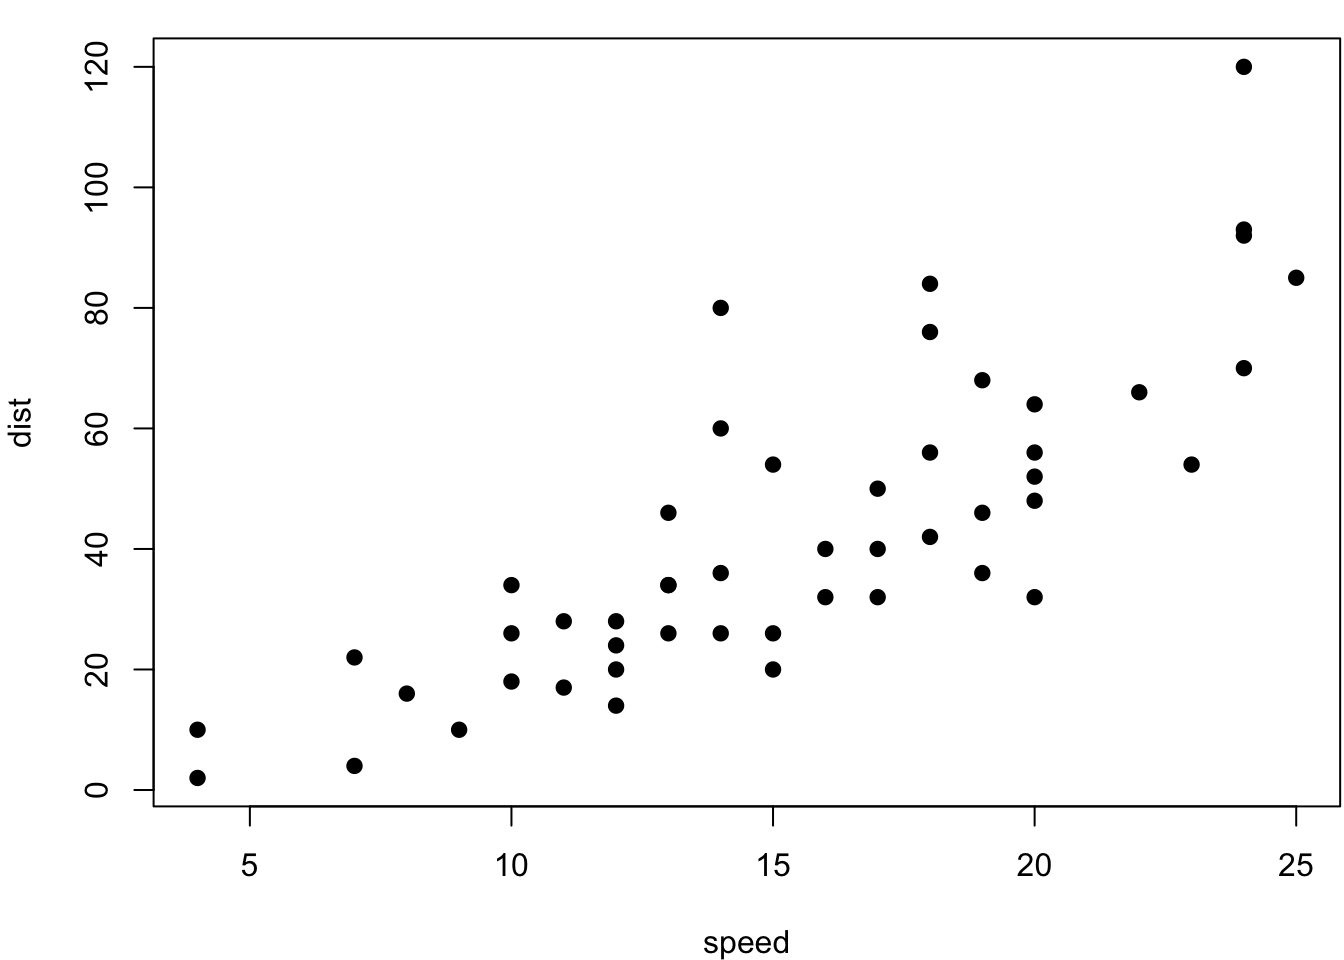
\includegraphics[width=0.9\linewidth]{bookdown_files/figure-latex/hello-1} \caption{雷猴啊,散点图!}\label{fig:hello}
\end{figure}

\begin{Shaded}
\begin{Highlighting}[]
\NormalTok{knitr}\OperatorTok{::}\KeywordTok{kable}\NormalTok{(}
  \KeywordTok{head}\NormalTok{(iris), }\DataTypeTok{caption =} \StringTok{'雷猴啊,iris 数据!'}\NormalTok{,}
  \DataTypeTok{booktabs =} \OtherTok{TRUE}
\NormalTok{)}
\end{Highlighting}
\end{Shaded}

\begin{table}[t]

\caption{\label{tab:iris}雷猴啊,iris 数据!}
\centering
\begin{tabular}{rrrrl}
\toprule
Sepal.Length & Sepal.Width & Petal.Length & Petal.Width & Species\\
\midrule
5.1 & 3.5 & 1.4 & 0.2 & setosa\\
4.9 & 3.0 & 1.4 & 0.2 & setosa\\
4.7 & 3.2 & 1.3 & 0.2 & setosa\\
4.6 & 3.1 & 1.5 & 0.2 & setosa\\
5.0 & 3.6 & 1.4 & 0.2 & setosa\\
\addlinespace
5.4 & 3.9 & 1.7 & 0.4 & setosa\\
\bottomrule
\end{tabular}
\end{table}

就这样,你可以一直编下去,直到编不下去。

\hypertarget{section-6}{%
\chapter{特色功能展示}\label{section-6}}

\hypertarget{section-7}{%
\section{本地和服务器同步}\label{section-7}}

\hypertarget{section-8}{%
\section{合作编辑}\label{section-8}}

\hypertarget{section-9}{%
\section{历史版本}\label{section-9}}

\hypertarget{section-10}{%
\section{参考文献整合}\label{section-10}}

张老爷子

话说张老爷子写了一首诗:

\begin{quote}
姑苏开遍碧桃时,邂逅河阳女画师。\\
红豆江南留梦影,白苹风末唱秋词。
\end{quote}

彭大将领

貌似大家都喜欢用白萍风这个意境。又如彭玉麟的对联:

\begin{quote}
凭栏看云影波光,最好是红蓼花疏、白苹秋老;\\
把酒对琼楼玉宇,莫孤负天心月到、水面风来。
\end{quote}

嘿,玛尼玛尼哄。

\hypertarget{section-11}{%
\chapter{订阅费用}\label{section-11}}

\url{https://www.overleaf.com/user/subscription/plans}

张老爷子

话说张老爷子写了一首诗:

\begin{quote}
姑苏开遍碧桃时,邂逅河阳女画师。\\
红豆江南留梦影,白苹风末唱秋词。
\end{quote}

彭大将领

貌似大家都喜欢用白萍风这个意境。又如彭玉麟的对联:

\begin{quote}
凭栏看云影波光,最好是红蓼花疏、白苹秋老;\\
把酒对琼楼玉宇,莫孤负天心月到、水面风来。
\end{quote}

嘿,玛尼玛尼哄。

\hypertarget{section-12}{%
\chapter{特色功能展示}\label{section-12}}

\hypertarget{section-13}{%
\section{本地和服务器同步}\label{section-13}}

\hypertarget{section-14}{%
\section{合作编辑}\label{section-14}}

\hypertarget{section-15}{%
\section{历史版本}\label{section-15}}

\hypertarget{section-16}{%
\section{参考文献整合}\label{section-16}}

张老爷子

话说张老爷子写了一首诗:

\begin{quote}
姑苏开遍碧桃时,邂逅河阳女画师。\\
红豆江南留梦影,白苹风末唱秋词。
\end{quote}

彭大将领

貌似大家都喜欢用白萍风这个意境。又如彭玉麟的对联:

\begin{quote}
凭栏看云影波光,最好是红蓼花疏、白苹秋老;\\
把酒对琼楼玉宇,莫孤负天心月到、水面风来。
\end{quote}

嘿,玛尼玛尼哄。

\hypertarget{section-17}{%
\chapter{其他工具}\label{section-17}}

这里介绍一些可以提高LaTeX写作效率的其他工具

\hypertarget{section-18}{%
\section{输入公式}\label{section-18}}

mathpix

可以很方便的将图片公式转成LaTex形式,手写笔记不太乱的话也是可以识别的.

\url{https://mathpix.com}

\hypertarget{section-19}{%
\section{输入表格}\label{section-19}}

\hypertarget{excel2latex}{%
\subsection{Excel2LaTeX}\label{excel2latex}}

可以在Excel中合并好单元格,导出tex的表格.

\url{https://github.com/krlmlr/Excel2LaTeX/releases}

\hypertarget{xtable}{%
\subsection{xtable包}\label{xtable}}

在R中进行模拟时,将结果输出至LaTeX可以利用这个包中的xtable函数.

\url{https://cran.r-project.org/web/packages/xtable/index.html}

\begin{Shaded}
\begin{Highlighting}[]
\NormalTok{xtable}\OperatorTok{::}\KeywordTok{xtable}\NormalTok{(}\KeywordTok{matrix}\NormalTok{(}\KeywordTok{rnorm}\NormalTok{(}\DecValTok{12}\NormalTok{),}\DecValTok{3}\NormalTok{,}\DecValTok{4}\NormalTok{))}
\end{Highlighting}
\end{Shaded}

\begin{verbatim}
## % latex table generated in R 3.6.0 by xtable 1.8-4 package
## % Fri May 31 15:57:39 2019
## \begin{table}[ht]
## \centering
## \begin{tabular}{rrrrr}
##   \hline
##  & 1 & 2 & 3 & 4 \\ 
##   \hline
## 1 & 0.81 & 2.71 & 0.77 & 1.15 \\ 
##   2 & -2.27 & -0.94 & -0.40 & -0.89 \\ 
##   3 & 1.75 & -0.21 & 0.42 & -1.41 \\ 
##    \hline
## \end{tabular}
## \end{table}
\end{verbatim}

\hypertarget{latex}{%
\section{LaTeX中合并单元格}\label{latex}}

\url{http://www.tablesgenerator.com/\#}

\hypertarget{section-20}{%
\chapter{一些模板}\label{section-20}}

\hypertarget{section-21}{%
\section{学位论文模板}\label{section-21}}

\url{https://github.com/ustctug/awesome-latex-thesis}

\hypertarget{elegantlatex}{%
\section{ElegantLaTeX}\label{elegantlatex}}

\url{https://github.com/ElegantLaTeX}

\hypertarget{beamer}{%
\section{beamer模板}\label{beamer}}

\url{http://deic.uab.es/~iblanes/beamer_gallery/index_by_theme.html}

\url{https://www.namsu.de/latex/themes/outer.html}

\cleardoublepage

\hypertarget{appendix-}{%
\appendix \addcontentsline{toc}{chapter}{\appendixname}}


\hypertarget{sound}{%
\chapter{余音绕梁}\label{sound}}

呐,到这里朕的书差不多写完了,但还有几句话要交待,所以开个附录,再啰嗦几句,各位客官稍安勿躁、扶稳坐好。

\bibliography{book.bib,packages.bib}

\backmatter
\printindex

\end{document}
